\documentclass{beamer}
\usepackage{ngerman}
\usepackage[utf8]{inputenc}
\usepackage{pgf}
\usepackage{verbatim}
\usepackage{listings}
\usepackage[]{hyperref} 
\usepackage{multicol}
\beamertemplatenavigationsymbolsempty

\usetheme{Szeged}

\title{HadoopDB\\ ein großer Schritt in die falsche Richtung}
\subtitle[]{Seminar 01912\\ Sommersemester 2011}
\date{\today}
\author[T. Koch]{Thomas Koch}
\institute[Fernuni Hagen]{Lehrgebiet Datenbanksysteme für neue Anwendungen\\ Fernuniversität Hagen}

\begin{document}
  \begin{frame}
    \titlepage
  \end{frame}

  \begin{frame}
    \tableofcontents{}
  \end{frame}

\section{HadoopDB}

\begin{frame}{Anforderungen}
  \begin{itemize}
    \item Performanz
    \item Fehlertoleranz
    \item Heterogene Server
    \item Flexible / Erweiterbare Abfrageschnittstelle
  \end{itemize}
  (Energieeffizienz?)
\end{frame}

\begin{frame}
  \begin{tabular}{r c c}
     & Parallele DBs & MapReduce \\
     Performanz & ++ & ? \\
     Fehlertoleranz & -- & ++ \\
     Heterogene Server & -- & ++ \\
     Abfrageschnittstelle & ++ (?) & + \\
  \end{tabular}
\end{frame}

\begin{frame}{Architektur}
  \begin{center}
    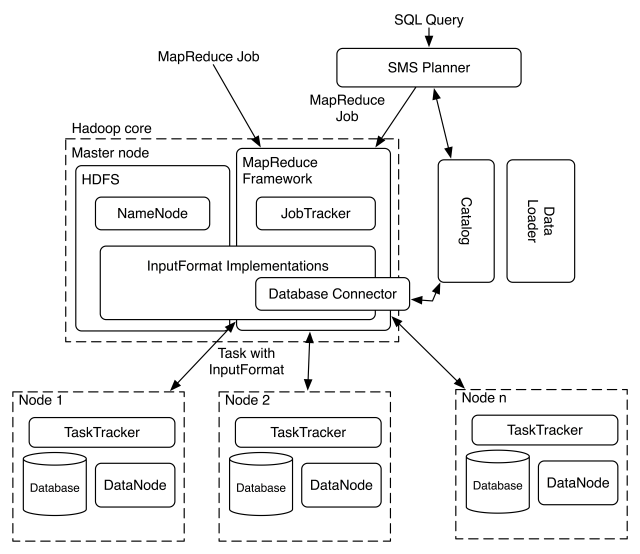
\includegraphics[width=0.7\textwidth]{../ausarbeitung/images/hadoopdb-arch.png}    
  \end{center}
\end{frame}

\begin{frame}{Datenladephase}
  \begin{enumerate}
    \item globaler Hasher (2r, 2w + 1 network copy)
    \item Export ins lokale Dateisystem (1r, 1w)
    \item lokaler Hasher (1r, 1w)
    \item Import in lokale Datenbank (1r, 1w + Indizes)
  \end{enumerate}
  \pause
  5x lesen, 5x schreiben
\end{frame}

\begin{frame}[fragile]{SQL-MapReduce-SQL Planer}
\begin{verbatim}
SELECT YEAR(saleDate), SUM(revenue)
FROM sales GROUP BY YEAR(saleDate)
\end{verbatim}
\end{frame}

\begin{frame}{SQL-MapReduce-SQL Planer}
  \begin{center}
    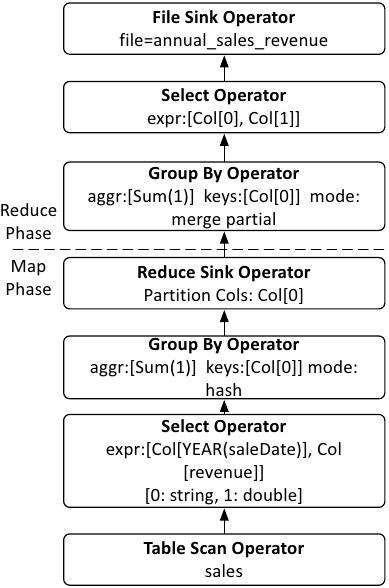
\includegraphics[height=0.8\textheight]{../ausarbeitung/images/hadoopdb-reduce-map-phase_a.png}    
  \end{center}
\end{frame}
\begin{frame}{SQL-MapReduce-SQL Planer}
  \begin{center}
    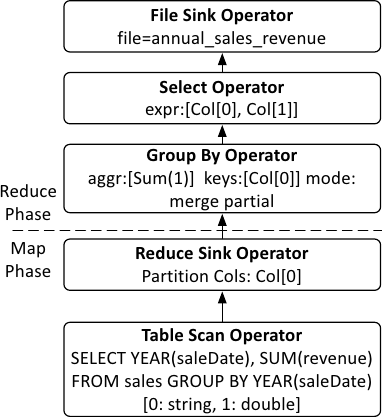
\includegraphics[height=0.8\textheight]{../ausarbeitung/images/hadoopdb-reduce-map-phase_c.png}    
  \end{center}
\end{frame}
\begin{frame}{SQL-MapReduce-SQL Planer}
falls per YEAR(saleDate) partitioniert wurde:
  \begin{center}
    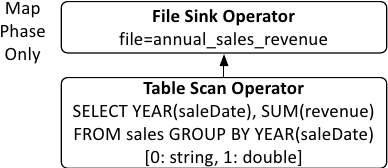
\includegraphics[height=0.3\textheight]{../ausarbeitung/images/hadoopdb-reduce-map-phase_b.png}    
  \end{center}
\end{frame}

\begin{frame}{weitere HadoopDB Komponenten}
  \begin{itemize}
  \item Datenbank Connectoren
  \item Catalog:
    \begin{itemize}
    \item Datenbankverbindungsparameter
    \item Metainformationen der Tabellen
    \item Speicherorte von Replikationen
    \item Partitionseigenschaften
    \end{itemize}
  \end{itemize}
\end{frame}

\begin{frame}[fragile]{Grep Task}
  \begin{columns}
    \begin{column}{0.3\textwidth}
\begin{verbatim}
SELECT * FROM Data
 WHERE
field LIKE '%XYZ%';
\end{verbatim} 
Compression?
    \end{column}
    \begin{column}{0.7\textwidth}
      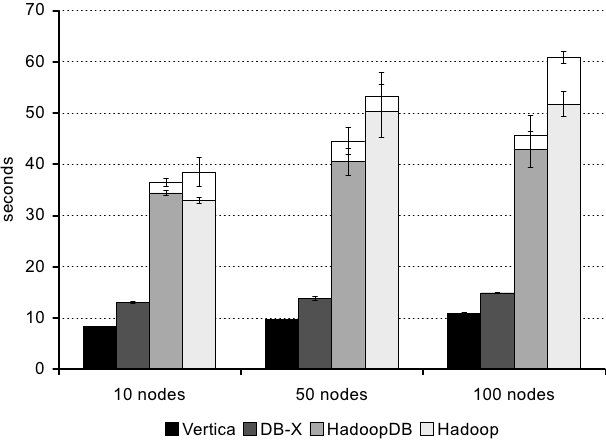
\includegraphics[width=\textwidth]{../ausarbeitung/images/diagram_grep_task.png}
    \end{column}
  \end{columns}
\end{frame}

\begin{frame}[fragile]{Schemas der analytischen Tasks}
  \begin{multicols}{2}
\begin{verbatim}
CREATE TABLE Documents
( url VARCHAR(100) 
      PRIMARY KEY,
  contents TEXT 
);

CREATE TABLE Rankings 
( pageURL VARCHAR(100) 
          PRIMARY KEY,
  pageRank INT,
  avgDuration INT 
);
\end{verbatim}    

\begin{verbatim}
CREATE TABLE UserVisits
( sourceIP VARCHAR(16),
  destURL VARCHAR(100),
  visitDate DATE,
  adRevenue FLOAT,
  userAgent VARCHAR(64),
  countryCode VARCHAR(3),
  languageCode VARCHAR(6),
  searchWord VARCHAR(32),
  duration INT 
);
\end{verbatim}
  \end{multicols}
\end{frame}

\begin{frame}[fragile]{Selection Task}
  \begin{columns}
    \begin{column}{0.3\textwidth}
\begin{verbatim}
SELECT pageUrl,
pageRank 
FROM Rankings
WHERE pageRank > 10;
\end{verbatim} 
    \end{column}
    \begin{column}{0.7\textwidth}
      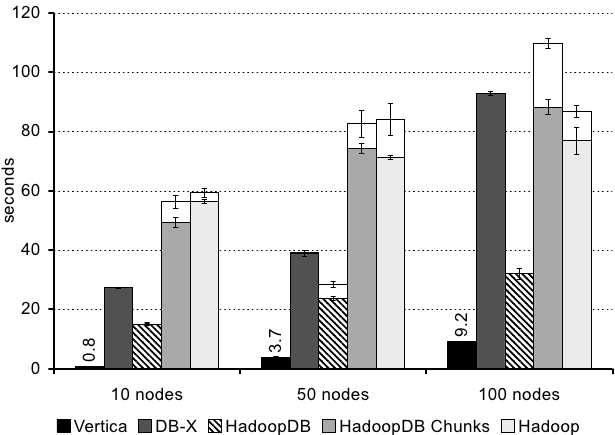
\includegraphics[width=\textwidth]{../ausarbeitung/images/diagram_selection_task.png}
    \end{column}
  \end{columns}
\end{frame}

\begin{frame}[fragile]{Aggregation Task}
  \begin{columns}
    \begin{column}{0.3\textwidth}
\begin{verbatim}
SELECT sourceIP,
SUM(adRevenue)
FROM UserVisits 
GROUP BY sourceIP;
\end{verbatim} 
    \end{column}
    \begin{column}{0.7\textwidth}
      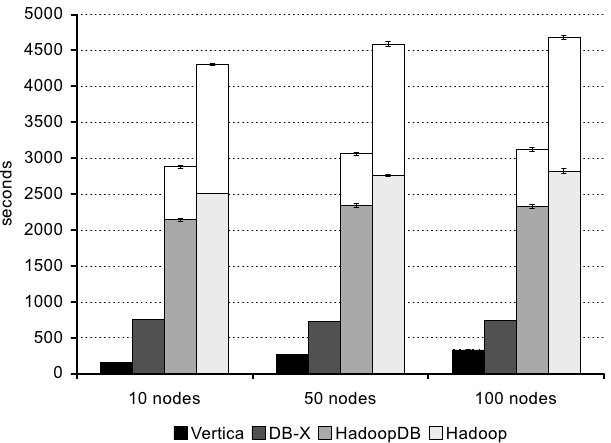
\includegraphics[width=\textwidth]{../ausarbeitung/images/diagram_aggregation_task.png}
    \end{column}
  \end{columns}
\end{frame}

\begin{frame}[fragile]{Join Task}
  \begin{columns}
    \begin{column}{0.6\textwidth}
\begin{verbatim}
SELECT sourceIP, COUNT(pageRank),
SUM(pageRank), SUM(adRevenue)
FROM Rankings AS R,
     UserVisits AS UV
WHERE
R.pageURL = UV.destURL AND
UV.visitDate BETWEEN
  '2000-01-15' AND '2000-01-22'
GROUP BY UV.sourceIP;
\end{verbatim} 
    \end{column}
    \begin{column}{0.4\textwidth}
      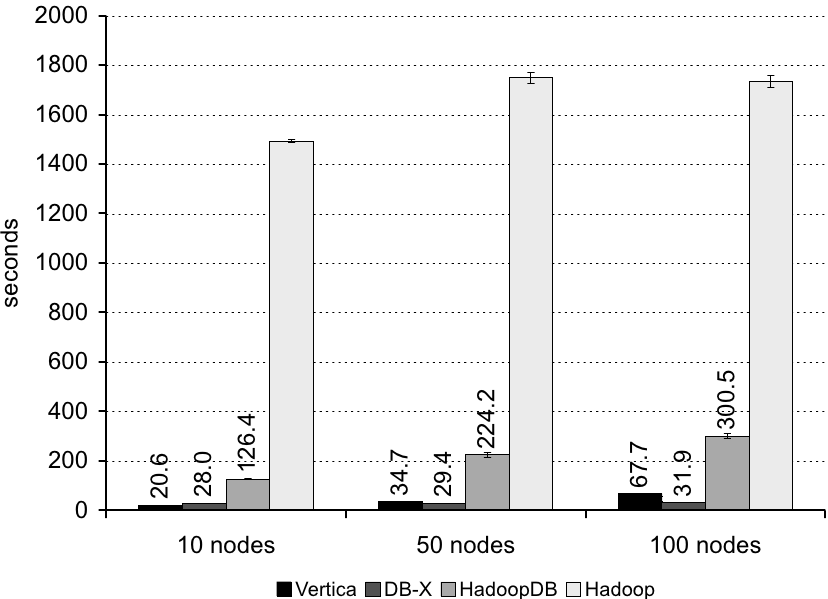
\includegraphics[width=\textwidth]{../ausarbeitung/images/diagram_join_task.png}
    \end{column}
  \end{columns}
\end{frame}

\begin{frame}{Linkgraph-Invertier Task}
  HTML parsen, Links extrahieren, Inlinks für Seiten zählen.
  
  Musterbeispiel für MapReduce!
\end{frame}

\begin{frame}{Diskussion}
  \begin{itemize}
  \item unrealistische Benchmarks
  \item sehr kleine Anzahl Server
  \item Fehlbedienung von Hadoop?
  \item keine richte Fault-Tolerance
  \item separate Read-Only Datenbank
  \end{itemize}
\end{frame}

\begin{frame}{Praktische Evaluation - Feedback}
  \begin{itemize}
  \item \textless 10 unabhängige Google Treffer
  \item 15 (4 letztes Jahr) Mails auf PostgreSQL Liste
  \item 22 Revisions in Subversion
  \end{itemize}
  \pause
  \ldots obwohl es \textbf{Hadoop}DB heißt!
\end{frame}

\begin{frame}{Praktische Evaluation}
  Kombination von mind. 2 komplizierten Systemen:

  Hadoop (+Hive) + Datenbank (PostgreSQL)
\end{frame}

\section{Hive}

\begin{frame}{Überblick}
  \begin{itemize}
    \item entwickelt von FaceBook
    \item SQL ähnliche Abfragesprache
    \item Ausführung als DAG von MapReduce Jobs
  \end{itemize}
\end{frame}

\begin{frame}{Datenmodell}  
  \begin{itemize}
  \item Tabellen
  \item Partitionen
  \item Buckets
  \end{itemize}
\begin{displaymath}
  /wh/\underbrace{daily\_status}_{\text{table name}}/\underbrace{ds=20090101/ctry=US}_{\text{nested partitions}}/\underbrace{0001}_{\text{bucket}}
\end{displaymath}
\end{frame}

\begin{frame}{Architektur}
  \begin{center}
    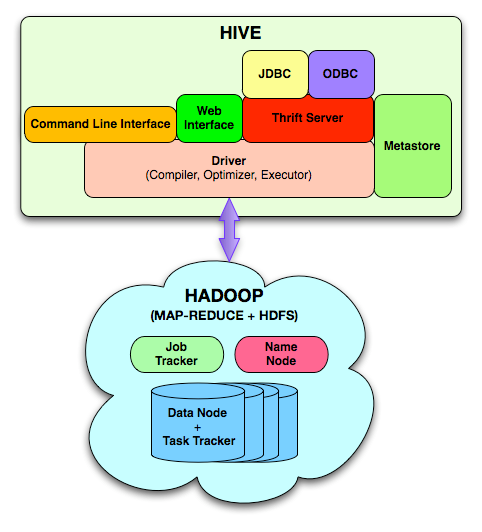
\includegraphics[height=\textheight]{../ausarbeitung/images/hive-architecture.png}    
  \end{center}
\end{frame}

\begin{frame}{Hive-Metastore}
  \begin{itemize}
  \item Schema: browse, query parsing
  \item (geplant) Statistiken: Optimierung
  \end{itemize}
  Demnächst: HCatalog
\end{frame}

\begin{frame}{Hive-Compiler}
  \begin{enumerate}
\item Query String $\rightarrow$ Parsebaum
\item $\rightarrow$ interne Queryrepresentation +
  \begin{itemize}
  \item Verifikation gegen Metastore
  \item SELECT * expandieren
  \item Typcheck bzw. conversion
  \end{itemize}
\item $\rightarrow$ logischer Operatorbaum
\item Optimierer
\item $\rightarrow$ MapReduce jobs
\end{enumerate}
  
\end{frame}

\begin{frame}[fragile]{Vergleich mit SQL}
  \begin{itemize}
    \item standard Datentypen + Array, Maps + user programed
    \item kein update, delete, insert into
    \item user defined (aggregation) functions
    \item Mehrere INSERTs aus einem SELECT
  \end{itemize}
\pause
\begin{verbatim}
FROM (SELECT ...) subq1
INSERT TABLE a SELECT subq1.xy, subq1.xz
INSERT TABLE b SELECT subq1.ab, subq1.xy
\end{verbatim}
\end{frame}
\end{document}